\chapter{Detector Design}\label{c:det-design}

This chapter describes the design and choice of parameters for the \TES\ bolometers that are used in the \Imager.

\section{Parameter Choice For Our Bolometers} \label{sec:det-parm-choice}

The primary parameters to be chosen when designing a \TES\ bolometer are the superconducting critical temperature $T_c$, the thermal conductance $G$, and the \TES\ island heat capactiy $C$.
These parameters are interrelated, and so cannot be chosen entirely independently of each other.
Some of the factors to consider are:
\begin{itemize}
  \item Detector noise scales with $\sqrt{T_c^2 G}$, so that lower values of $G$ and $T_c$ are better
  \item The saturation power of the \TES\ detector scales roughly like $G T_c$, so that if $G$ and $T_c$ are too small, the optical power falling on the detector will raise the temperature of the membrane above $T_c$, causing the device to not work.
    % do i talk about saturation power in ch 3? if not, I should!
  \item $T_c$ must be chosen to be higher than the acheivable bath temperature, and the bath temperature also affects the saturation power.
  \item The targetted detector time constant $\tau_{eff}$ depends not only on the detector natural time constant $\tau = G / C$ but also on the values of \Loop and $\beta_I$ at the chosen bias point.
        The loop gain depends primarily on the detector $\alpha$, but also on the saturation power.
\end{itemize}

The following subsections outline the choice of $T_b$, $T_c$, $G$ and $C$ for the detectors in the first 251-detector sub-array.

xxx say something about no attempt to shape transition - we get whatever alpha we get. no need to slow down trans, which is what normal metal bars do.

\subsection{Choice of $T_b$ and $T_c$}

The relationship between detector noise and saturation power can be examined in more detail.
From \eqnref{eqn:ch3-g-fit} we have
\begin{equation} \label{eqn:ch5-psat}
P_{sat} = \frac{G T_c}{n}\left(1 - \left(\frac{T_b}{T_c}\right)^n\right).
\end{equation}
This can be solved for $G$ and substituted into the expression for \TES\ thermal fluctuation noise in \tableref{tab:tes-noise}, leading to
\begin{equation} \label{eqn:ch5-tes-noise}
S^2_{TFN} = \frac{n F(T_0, T_b) T_0 / T_b}{1-(T_b/T_c)^n} 4 k_B T_b P_{sat}.
\end{equation}
The \TES\ temperature $T_0$ only appears in the pre-factor, which depends only on the power-flow index $n$ and the ratio $T_b/T_0$.
This means that for fixed $P_{sat}$ and $T_b$, the ratio $T_c/T_b$ that gives the lowest detector noise depends only on $n$ and the form of $F$.
For values of $n$ in the range 3--4, this optimal ratio is $T_c \approx 1.8 T_b$, while the pre-factor itself is \abt{3.7}.

As discussed in \sectionref{sec:ch4-opt-eff}, the predicted loading on the \Imager's detectors is \SI{180}{\pW} and the photon noise from this load is \Pnoisef{0.85}.
Choosing a safety factor of 3 so that $P_{sat} = 3 \times \SI{200}{\pW}$, and targeting detector noise equal to \SI{50}{\percent} of the photon (so that total noise is a factor of $\sqrt{1.5} = 1.22$ higher than photon noise) we find that in order for the detector noise to be below the predicted photon noise we require
\begin{equation}
  T_b < \frac{1}{3.7} \frac{\NEPph^2}{4 k_B P_{sat}} =
        \frac{1}{3.7} \frac{0.5 \times (\num{0.85e-15})^2}{4 \times \SI{1.38e-23}{\J\per\K} \times 3 \times \SI{180}{\pW}} = 
        \SI{3.6}{\K}
\end{equation}
It would seem that we should be able to run the system off of a Pulse Tube Cooler.

However, this leaves very little margin for error in the design and implementation of the system, so for the \Imager\ we chose to use a \He4-sorption fridge to set the bath temperature.

The \Imager's base bath temperature under optical load is \SI{970} (see \sectionref{xxx}).
The initial hopes for performance of the \He4-sorption fridge were that it's base temperature would be ~\SI{650}{\mK}, implying an ideal $T_c$ of \abt{\SI{1.2}{\K}}.
This is a convenient $T_c$ because it is the critical temperature of elemental Al \cite{xxx}, so Al was chosen as the \TES\ material.

In practice, it was discovered during testing of Al prototype detectors that the base temperature of the system was \SI{950}{\mK} under optical load, so that a higher $T_c$ could lead to better noise performance.
However, in order to change as little as possible between the prototype detectors and the first sub-array, I decided to continue using Al.

\subsection{Choice of $G$}

\tableref{tab:ch5-proto-parms} lists the measured properties and parameters of the prototype detectors.
These detectors had $P_{sat}$ at $T_b = \SI{970}{\mK}$, 5.1 times higher than the predicted optical load and 6.1 times the measured optical load.
A safety factor of 5--6 is overly conservative, so for the sub-array I decided to target a $G$ value of \SI{3.8}{\nW\per\K}, for a safety factor of 3.9 -- 4.7.

\begin{table*}
\centering
\caption{
  Measured Properties of Prototype Detectors.
  The methods and procedures used to measure these properties were the same as described for the sub-array in \chapterref{c:det-array}.
} 
\label{tab:ch5-proto-parms}
\begin{tabular}{l c}
\toprule
  Detector Property &  {Value} \\
\midrule
  $T_c$                 & \SI{1.2}{\K} \\
  $R_n$                 & \SI{3.4}{\mOhm} \\
  $n$                   & 3.9 \\
  $G$                   & \SI{5}{\nW\per\K} \\
  $\tau$                & \SI{12}{\ms} \\
  $\tau_{eff} (typical)$ & \SI{4}{\ms} \\
  $C = G \tau $         & \SI{60}{\pJ\per\K} \\
  $P_{opt}$              & \SI{150}{\pW\per\K} \\
  $\eta_{tot}$           & 0.25 \\
  $P_{sat,970}$          & \SI{920}{\pW} \\
\bottomrule
\end{tabular}
\end{table*}

\subsection{Choice of $C$}

The detector's heat capacity $C$ is chosen to target a specific natural time constant $\tau$ once $G$ is chosen.
$\tau_{eff}$ in the prototype detectors was higher than the desired value of \SI{1}{\ms}.
To reduce risk of problems such as instability with the sub-array detectors, I decided to reduce $C$ to \SI{30}{\pJ\per\K}, which would give $\tau = \SI{8}{\ms}$.
As long as \Loop and $\beta_I$ at the operating bias point did not change, this would lead to $\tau_{eff} = \SI{2.6}{\ms}$.

\section{Detailed Detector Design} \label{sec:ch5-det-design}

The \Imager's detectors are fabricated using standard lithographic clean-room techniques on Si wafers.
In order to achieve the targetted $G$ and $C$ values the detectors are located on a suspended SiN membrane which is connected to the rest of the Si wafer by a set of thin ``legs''.
\figref{xxx} shows a cross-sectional schematic of the detectors, showing that they are suspended with no Si beneath them, as well as a labeled photograph of a prototype detector (the sub-array detectors are identical except for the length of the legs and the thickness of some of the layers; see \tableref{tab:ch5-det-dims}).

xxx photo / cross-section figure

The detectors are fabricated on \SI{275}{\um} thick double-side-polished degenerate (Boron P-type) Si wafers.
A layer of SiO2 is grown on top of the silion, followed by a layer of SiN, prior to the main fabrication steps.
During fabrication the \TES\, Nb wiring leads, PdAu absorber, and Au heat-capacity ring are laid down, as well as an additional layer of insulator to allow wiring layers to cross over each other.
The SiN and SiO2 is removed from the areas between the legs, and then a Deep Reactive Ion Etch process is used to remove all silicon from behind the detector membrane.
This etch process does not remove SiN or SiO2, so that the legs, which still have SiN, are left in place.
The result is a susepended membrane connected to the rest of the wafer by a set of ``legs'' which provide the thermal conductance $G$.

\tableref{tab:ch5-det-dims} lists dimensions for both the prototype and sub-array detectors.

The leg geometry of the prototype detectors was based on a set of measurements taken at \NIST\ on SiN membranes at temperature around \SI{1}{\K}.
the leg geometry for the sub-array detectors was based on simple scaling of the prototype detecctors to the target $G$ of \SI{3.8}{\nW\per\K}.
This scaling was slightly complicated by the change in thickness of the SiO2 layers, which was made in order to add additional protection to the wiring laayers and better balance stress on the relieved membranes.
Assuming that $G$ scales linearly with the $A/L$ of the legs, the sub-array $G$ should be
\begin{align}
  G_{sub} & = G_{proto} \frac{A_{sub}}{A_{proto}} \frac{l_{proto}}{l_{sub}} \\
         & = G_{proto} \frac{(500 + 250 + 200)(11)}{(500 + 120 + 120)(11)} \frac{40}{67} \\
         & = \SI{5.0}{\nW\per\K} \times 1.28 \times 0.597 \\
         & = \SI{3.8}{\nW\per\K} 
\end{align}

\begin{table*}
\centering
\caption{
  Dimensions of prototype and sub-array detectors.
  The values shown for the sub-array detectors are those that are different from the prototypes; all other sub-array dimensions are the same as for the prototypes.
} 
\label{tab:ch5-det-dims}
\begin{tabular}{l c c}
\toprule
  Detector Dimension &  {Prototype} & Sub-Array \\
\midrule
  \TES\ Size           & $\SI{64}{\um} \times \SI{70}{\um}$ & \\
  \TES\ Thickness      & \SI{250}{\nm}       & \SI{180}{\nm} \\
  SiN Thickness        & \SI{500}{\nm}       & \\
  SiO2 Base Thickness  & \SI{120}{\nm}       & \SI{250}{\nm} \\
  SiO2 Cover Thickness & \SI{120}{\nm}       & \SI{200}{\nm} \\
  Number of Legs       & 8                   & \\
  Leg Length           & \SI{40}{\um}        & \SI{67}{\um} \\
  Leg Width            & \SI{11}{\um}        & \\
  Gold Ring Area       & $(\SI{393}{\um})^2$ & \\
  Gold Ring Thickness  & \SI{2000}{\nm}      & \SI{1000}{\nm} \\
  Nb Lead Width        & \SI{6}{\um}         & \\
  Nb Lead Thickness    & \SI{200}{\nm}       & \\
  PdAu Thickness       & \SI{20}{\nm}        & \\
\bottomrule
\end{tabular}
\end{table*}

\tableref{xxx} shows contributions to the heat capactiy from all components of the bolometer.
The membrane and Al \TES\ alone have insufficient heat capacity, so an Au ring was added to provide the targetted heat capacity.
The total heat capacity is dominated by the Au ring.

\begin{table*}
\centering
\caption{
  Contributions to total heat capacity of sub-array detectors.
  Note that the Debye contribution for Au at \SI{1.2}{\K} is still significant, so can not be ignored.
} 
\label{tab:ch5-det-dims}
\begin{tabular}{l S S S l}
\toprule
  Component & {Volume ($10^{-9}$\,\si{\cm^3})} & {$C_V$ (\si{\uJ\per\K\per\cm^3})} & {$C_{tot}$ (\si{\uJ\per\K})} & Source \\
\midrule 
    SiN & 203.6 &   1.0 &   0.2 & \cite{holmes_measurements_1998} \\ 
   SiO2 & 183.2 &   3.1 &   0.6 & \cite{zeller_thermal_1971,zink_specific_2004} \\ 
     Al &   0.8 & 196.8 &   0.2 & \cite{irwin_transition-edge_2005} \\ 
     Au & 154.4 & 161.3 &  24.9 & \cite{corak_atomic_1955} \\ 
\midrule 
  Total &       &       &  25.8 \\ 
\bottomrule
\end{tabular}
\end{table*}

\begin{figure*}
\centering
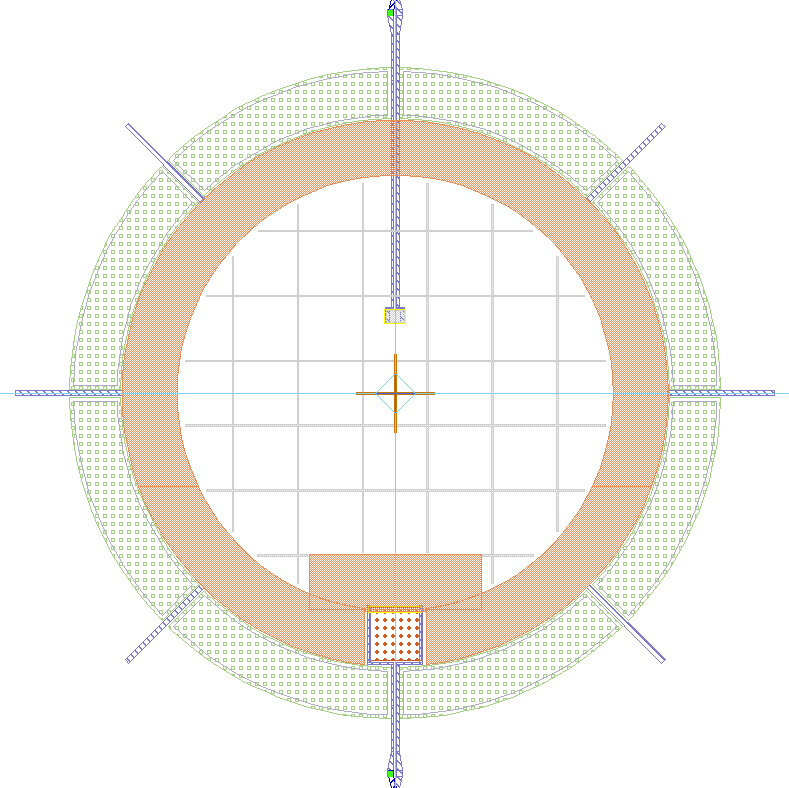
\includegraphics[height=2.5in]{images/ch5-det-layout.png}
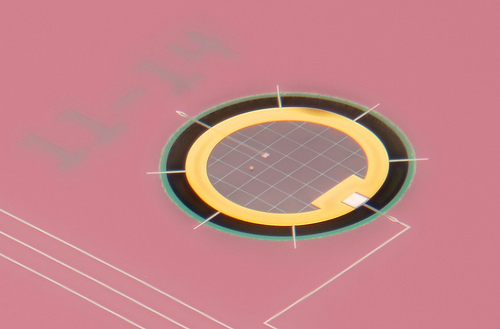
\includegraphics[height=2.5in]{images/ch5-single-pixel-500.jpg}
\caption{
  Layout of \Imager\ detectors.
}
\label{fig:ch5-det-layout}
\end{figure*}

\section{Detector Wafer Layout} \label{sec:ch5-layout}

\figref{fig:ch5-xxx} shows a photograph of the entire sub-array.
Bondpads for connecting to the detectors run along the top and right sides.
In the upper right and lower left corners are Au pads for connecting Au wirebonds to allow the wafer to be heat-sunk to the rest of the \SI{1}{\K} stage.
These corners also contain small bondpads for connecting to detector heaters.
While all detectors have heater resistors on their membrane, only the detectors along the left and lower edge have these resistors wired to bondpads.

The detectors are laid out on a square grid.
A hexagonal close-packed array would allow the same number of detetors to be placed on the array, but with feedhorns xxx larger.
The larger feedhorn size could have improved the spill over effieciency from xxx to xxx, leading to 

\section{Predicted Noise} \label{sec:ch5-predicted-noise}
